\documentclass[12pt, letterpaper, twoside]{article}
\usepackage[utf8]{inputenc}
\usepackage{amsmath}
\usepackage{amssymb}
\usepackage{graphicx}
\usepackage{epstopdf}
\usepackage{inputenc}
\usepackage{geometry}
\usepackage{booktabs}

\usepackage{tabularx}
\usepackage[english]{babel}
\newtheorem{theorem}{Theorem}

\geometry{left=2.5cm,right=2.5cm,top=2.5cm,bottom=2.5cm}
\usepackage{graphicx}
\graphicspath{ {./images/} }


\title{%
  Understanding Graph Theory \\
  
  \large In Application with Graph Coloring}
\author{ --insert name here-- \thanks{funded by the Kings University}}
\date{ May - August 2022 }


\begin{document}

\begin{titlepage}
\maketitle
\end{titlepage}

\begin{abstract}
Understanding Graph Theory. What is Graph Theory? 
Graph theory studies the mathematical structures used in moddelling the relationships between various elements.
The various elements, or nodes, are connected using edges. 
Nodes can be combined freely or with restrictions. In our study, we planted our attention on diverse restricted graph structures.
In line with graph theory, the application of Graph colouring became a primary outlet for research. Graph colouring is an essential application for studying restricted graphs. 
The colours act as labels for distinguishing elements on a constrained graph.
\end{abstract}

\begin{tabular}{l c p{.6\textwidth}}
\toprule
Terms           &                  & Definitions \\
\midrule
Degree &$:\Leftrightarrow$& The degree of a vertice refers to the number of connections it has.\\
Chromatic number &$:\Leftrightarrow$& The smallest number of colours needed to color a graph (for restricted graphs).\\
Connected Graph  &$:\Leftrightarrow$& A graph in which all nodes are connected with edges. \\
Restricted Graph  &$:\Leftrightarrow$& A graph in which connected adjacent nodes cannot have the same label/color.\\
Isomorphic Graph  &$:\Leftrightarrow$& A graph can take on different forms while having the same number of vertices and edges.\\
Bipartite Graph  &$:\Leftrightarrow$& A bipartite graph is a set of vertices placed into two disjoint sets restricting their vertices from connecting to adjacent vertices in the set.\\
Vertex Critical Graph  &$:\Leftrightarrow$& A critical vertex graph is a graph in which every vertex is a critical element, which will decrease the chromatic number on deletion.\\
Edge Critical Graph  &$:\Leftrightarrow$& A critical edge graph is a graph in which every edge is a critical element, which will decrease the chromatic number on deletion.\\

\bottomrule
\end{tabular}


\clearpage

\section{Introduction}
While misleading with its name, graph theory studies networks, relating connections found between a set of elements. These studies of networks find roots in graph colouring. 
Graph colouring is a unique problem in which connections made between elements ''vertices'' are assigned labels that prevent adjacent elements from sharing the same label.
Prominent uses of graph colouring can be identified with the colouring of maps, data mining, and networking and can even be found helpful in solving sudokus.

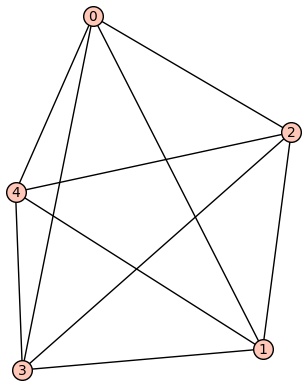
\includegraphics[scale=.35]{test}
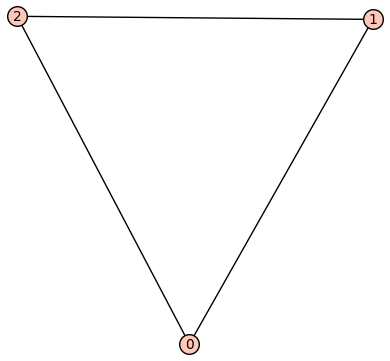
\includegraphics[scale=.35]{crit1}
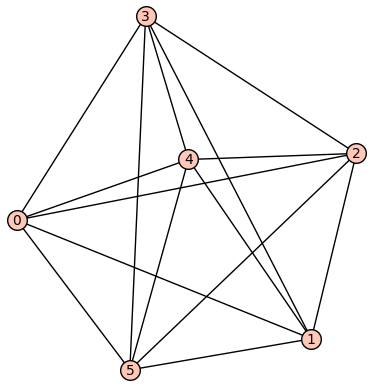
\includegraphics[scale=.35]{crit2}
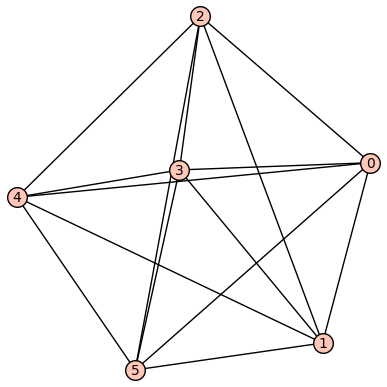
\includegraphics[scale=.35]{crit3}
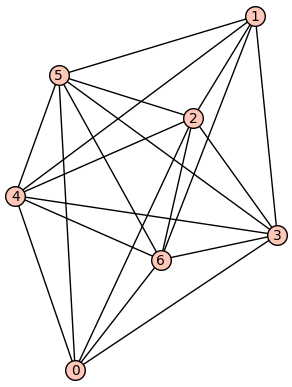
\includegraphics[scale=.35]{crit4}
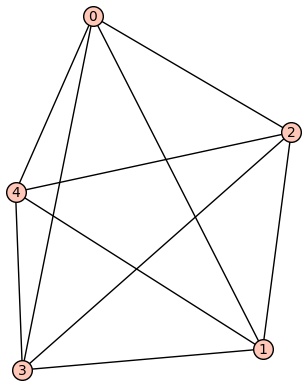
\includegraphics[scale=.35]{test}

\section{Critical Graphs}
Critical graphs are classified as being vertex or edge critical. This infers that not all vertex critical graphs will also be edge critical. To determine if a graph is critical, either an edge or vertex, when deleted, must be observed to change the graph's chromatic number. 
If deleting a vertex or edge results in an unchanged chromatic number, the graph is considered not critical.
Below are diagrams of critical graphs:

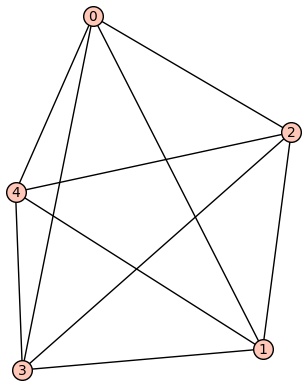
\includegraphics[scale=.35]{test}
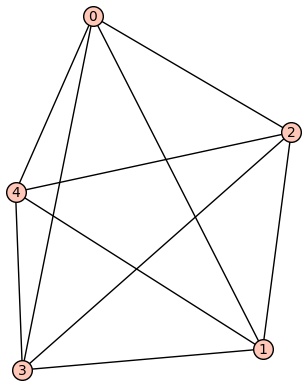
\includegraphics[scale=.35]{test}
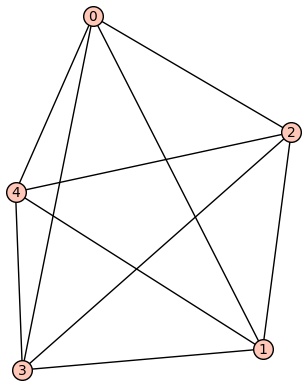
\includegraphics[scale=.35]{test}
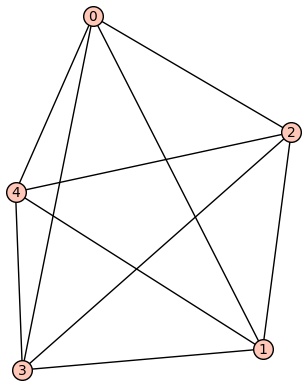
\includegraphics[scale=.35]{test}
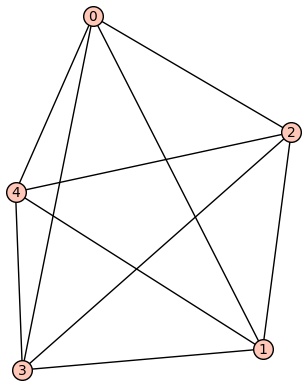
\includegraphics[scale=.35]{test}
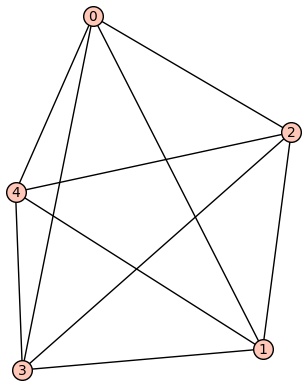
\includegraphics[scale=.35]{test}

\subsection{Exploring relationships between the degrees of a graph and its chromatic number}
The average degree of a graph appeared to have a seemingly unique relationship with the chromatic number. 
Interestingly, this relationship on the bipartite graph resulted in an asymptotic approach to a value of 2 as the number of vertices increased. 
While promising, this relationship appeared to have flaws with some graphs, resulting in values precisely one less than the chromatic number.  

\subsection{Finding efficiency in determining critical graphs}
The arduous process of deleting vertices in other to find criticality proves inefficient on time when analyzing graphs with larger vertices. 
However, what if such deletion of vertices becomes ''smart''?
The idea of first deleting vertices with a lesser or greater degree proved true in improving the time taken to classify critical graphs.
Through time analysis, deleting vertices with the largest degree first resulted in no time change, if not an increase. On the contrary, deleting vertices with the smallest degree resulted in faster criticality analysis.

\begin{theorem}
When determining what vertex to remove, removing vertices with the smallest degree first proves faster, as it eliminates non-critical graphs on the first deletion on average. 
\end{theorem}

Results (Graphs with 3 to 8 vertices)

\begin{tabularx}{0.9\textwidth} { 
  | >{\raggedright\arraybackslash}X 
  | >{\centering\arraybackslash}X 
  | >{\raggedleft\arraybackslash}X | }
  
\toprule
Deleting vertice with random degree & Deleting vertice with smallest degree & Deleting vertice with largest degree \\
\midrule

 20.96s & 12.71s & 21.45s \\
 \hline
 25.7s  & 13.09s  & 19.29s  \\
 \hline
 21.48s  & 14.55s  & 21.86s  \\
 \hline
 25.0s  & 15.06s  & 19.39s  \\
 \hline
 18.79s  & 14.48s  & 20.86s  \\

\hline
\end{tabularx}

\subsubsection{Using Neural Networks to classify critical graphs}
The application of neural networks became a potential game-changer for classifying graphs efficiently and quickly. I created a feed-forward neural network with four input features and two outputs. These select input features were the graph order (number of vertices), minimum graph degree, maximum graph degree and the chromatic graph number. 
These features created an interesting result, which sparked further exploration into the use of neural networks for classifying critical/non-critical graphs.
\\
\\[0.05in]

Results (Graphs with 3 to 8 vertices)

\begin{tabularx}{0.95\textwidth} { 
  | >{\raggedright\arraybackslash}X 
  | >{\raggedleft\arraybackslash}X 
  | >{\raggedleft\arraybackslash}X | }
  
\toprule
 & Test 1 & Test 2 \\
\midrule

 Loss & -0.06075938045978546 & -0.08965345472097397 \\
 \hline
 learning rate & 5e-06 & 5e-06  \\
 \hline
 Epoch Length & 1000 & 1000  \\
 \hline
 Actual Classification \\ 0 = Not Critical \\ 1 = Critical & 1, 1, 1, 0, 1, 0, 0, 1, 0, 1, 0, 0 & 1, 1, 0, 1, 1, 0, 0, 1, 0, 1, 0, 0  \\
 \hline
 Agent's Classification \\ 0 = Not Critical \\ 1 = Critical & 1, 0, 1, 0, 1, 0, 0, 1, 0, 1, 0, 0 & 1, 1, 0, 1, 1, 0, 0, 1, 0, 1, 0, 0  \\

\hline
\end{tabularx}

Promising result! Test 2, proving identical results.


\section{Deep Q-Learning Agent Classifies Critical Graphs}
Classifying graphs as critical using select features proved true potential, as results were very similar. However, the basis on which features were selected could potentially hinder the improvement of the model. 
It's frankly impossible to know the absolute best features to accurately classify graphs.
I decided to try something outright obvious; to feed the agent an input of the graph. Using a flattened matrix representation of the graph, the deep Q-earning agent derived its own patterns in an effort to maximize its reward. I awarded regards to the agent when its classifications were correct. Likewise, rewards were stripped on false classifications. 
This iterative process created an elaborated agent which classifies graphs using the graphs matrix.
It's interesting to note that training slowed down as the rounds increased. This is because new training rounds are started when the agent makes an error. But as the training continues, the agent makes fewer errors, resulting in longer rounds.
\\

Results (Graphs with Order 5)

\begin{tabularx}{0.9\textwidth} { 
  | >{\raggedright\arraybackslash}X 
  | >{\centering\arraybackslash}X 
  | >{\raggedleft\arraybackslash}X | }
  
\toprule
Agents Classification & Graph & Correct Classification \\
\midrule

 Critical: 0.0003316s & DFw & Critical \\
 \hline
 Critical: 0.0002816s  & DCw & Critical  \\
 \hline
 Critical: 0.0002756s  & DEw & Not Critical  \\
 \hline
 Not Critical: 0.0002849s & DQo & Not Critical  \\

\hline
\end{tabularx}
\\[0.075in]

Results (Graphs with Order 8)

\begin{tabularx}{0.9\textwidth} { 
  | >{\raggedright\arraybackslash}X 
  | >{\centering\arraybackslash}X 
  | >{\raggedleft\arraybackslash}X | }
  
\toprule
Agents Classification & Graph & Correct Classification \\
\midrule

 Critical: 0.0003307s &  & Critical \\
 \hline
 Critical: 0.0003133s & & Critical  \\
 \hline
  Critical: 0.0004377s &  & Critical \\
 \hline
 Critical: 0.0003135s & & Critical \\
 \hline
 Critical: 0.0003059s &  & Critical \\
 \hline

 Not Critical: 0.000324s &  & Not Critical  \\
 \hline
 Not Critical: 0.0003142s &  & Not Critical  \\
 \hline
 Not Critical: 0.0003021s &  & Not Critical  \\
 \hline
 Not Critical: 0.0002992s &  & Not Critical  \\
 \hline
 Not Critical: 0.0003014s &  & Not Critical  \\
 \hline

\hline
\end{tabularx}


Results (Graphs with Order 9)

\begin{tabularx}{0.9\textwidth} { 
  | >{\raggedright\arraybackslash}X 
  | >{\centering\arraybackslash}X 
  | >{\raggedleft\arraybackslash}X | }
  
\toprule
Agents Classification & Graph & Correct Classification \\
\midrule

 Critical: 0.0003803s &  & Critical \\
 \hline
 Critical: 0.0004981s & & Critical  \\
 \hline
  Critical: 0.0005579s &  & Critical \\
 \hline
 Critical: 0.000499s & & Critical \\
 \hline
 Critical: 0.0005002s &  & Critical \\
 \hline

 Not Critical: 0.0004976s &  & Not Critical  \\
 \hline
 Not Critical: 0.0005088s &  & Not Critical  \\
 \hline
 Not Critical: 0.0004992s &  & Not Critical  \\
 \hline
 Not Critical: 0.0383444s &  & Not Critical  \\
 \hline
 Not Critical: 0.000474s &  & Not Critical  \\
 \hline

\hline
\end{tabularx}


\section{Deep Q-Learning Agent Classifies Critical Graphs}
Classifying graphs as critical using select features proved true potential, as results were very similar. However, the basis on which features were selected could potentially hinder the improvement of the model. 





\subsection{Patterns with 5-critical circulent graphs}
Notable 









\end{document}
